\documentclass{article}
\usepackage[T1]{fontenc}
\usepackage[polish]{babel}
\usepackage[utf8]{inputenc}
\usepackage{graphicx}
\graphicspath{{images/}}
\usepackage{blindtext}
\usepackage{hyperref}
\usepackage{placeins}
\usepackage{caption}
\usepackage{subcaption}

\title{Generacja tekstów piosenek}
\author{Maciej Krzyżanowski, Sebastian Kutny, Tomasz Lewandowski}
\date{Kwiecień 2023}

\begin{document}

\maketitle

\tableofcontents

\newpage
\section{Wstęp}
Celem projektu było stworzenie modelu generującego tekst piosenki na podstawie wybranych danych jako tekstów innych utworów. Wykorzystaliśmy 2 metody: łańcuchy Markova oraz rekurencyjne sieci neuronowe. \\ \\ Projekt zawiera narzędzie "scraper" do pozyskiwania danych ze stron: 
\begin{itemize}
    \item \url{https://www.tekstowo.pl}
    \item \url{https://www.azlyrics.com}
\end{itemize}
Implementacja została wykonana w języku Python oraz wykorzystuje biblioteki: 
\begin{itemize}
    \item pandas
    \item BeautifulSoup
    \item nltk
    \item request
    \item queue
    \item re
\end{itemize}
Dostępna jest opcja łączenia zbiorów danych do jednego pliku w celu wykorzystania ich jednocześnie. \\ \\
Przed rozpoczęciem przetwarzania danych są one oczyszczane poprzez ujednolcenie wielkości liter, usunięcie niepotrzebnych znaków interpunkcyjnych, słów zakazanych (np:. określających składowe tekstu utworu) oraz wyrażeń ze szczególnymi znakami interpunkcyjnymi jako określających zawartość tekstu.
\\ \\
Tekst jest generowany jako dowolna liczba wersów o dowolnej ilości słow.
\newpage
\section{Łańcuchy Markova}
\subsection{Wstęp}
Łańcuchy Markova to matematyczny model służący do generowania tekstu lub sekwencji innych elementów, takich jak dźwięki lub obrazy. Ideą modelu jest analiza sekwencji istniejących elementów i wykorzystanie tych informacji do przewidywania, jakie elementy powinny pojawić się następnie. \\
\\
W przypadku generowania tekstu, łańcuchy Markova są zwykle stosowane do analizy sekwencji słów w tekście źródłowym i generowania nowych sekwencji słów na podstawie tych informacji. Proces zaczyna się od wyboru deterministycznego lub losowego początkowego stanu łańcucha, a następnie generowania kolejnych stanów na podstawie informacji o pradwopodobieństwie wystąpienia po sobie stanów w analizowanym tekście w kontekście poprzednio wygenerowanych stanów. Przykładowo, jeśli w tekście źródłowym po słowie "generator" często pojawia się słowo "piosenek", to model łańcucha Markova przypisze wysokie prawdopodobieństwo wystąpienia słowa "piosenek" po słowie "generator". \\
\\
Istnieją różne sposoby implementacji modelu łańcuchów Markova, ale zwykle opierają się one na analizie pewnej liczby poprzednich elementów, zwanej "stopniem" modelu. Na przykład, w przypadku modelu pierwszego stopnia, prawdopodobieństwo wystąpienia danego elementu zależy tylko od poprzedniego elementu, w modelu drugiego stopnia, prawdopodobieństwo zależy od dwóch poprzednich elementów, a w modelu trzeciego stopnia, prawdopodobieństwo zależy od trzech poprzednich elementów itd. Stopień łańcucha nazywamy N-gramem.\\
\\
W naszym projektcie N-gram jest parametryzowany i bazuje na N uprzednio wygenerowanych słowach w wersie, losując następne słowo na podstawie prawdopodobieństwa jego wystąpienia po N sekwencji słów uprzednio wygenerowanych. Dodatkowo przy każdym wersie o nieparzystym numerze podejmowana jest próba stworzenia rymującego się wersu na podstawie ostatniej sylaby poprzedniego. Najpierw znajdowane są wszystkie rymujące się zakończenia wersu niebędące ostatnim słowem poprzedniego, a następnie - jeśli takie istnieją - losujemy jedno z nich zamiast z wszyskich pozycji. Przy nieznalezieniu rymujących się słów generacja odbywa się tak jak w zwykłym wypadku. W praktyce szansa na stworzenie rymu jest mała i powinna rosnąć z ilością danych przetwarzanych przez model.\\
\\
Model łańcuchów Markova nie jest idealny i może generować sekwencje, które nie są sensowne lub poprawne gramatycznie. Dopiero przy wglądzie modeli w setki stanów wstecz oraz przy bardzo dużej ilości danych można wygenerować tekst podobny do pisanego przez człowieka. \\
\\
\begin{figure}[h]
    \centering
    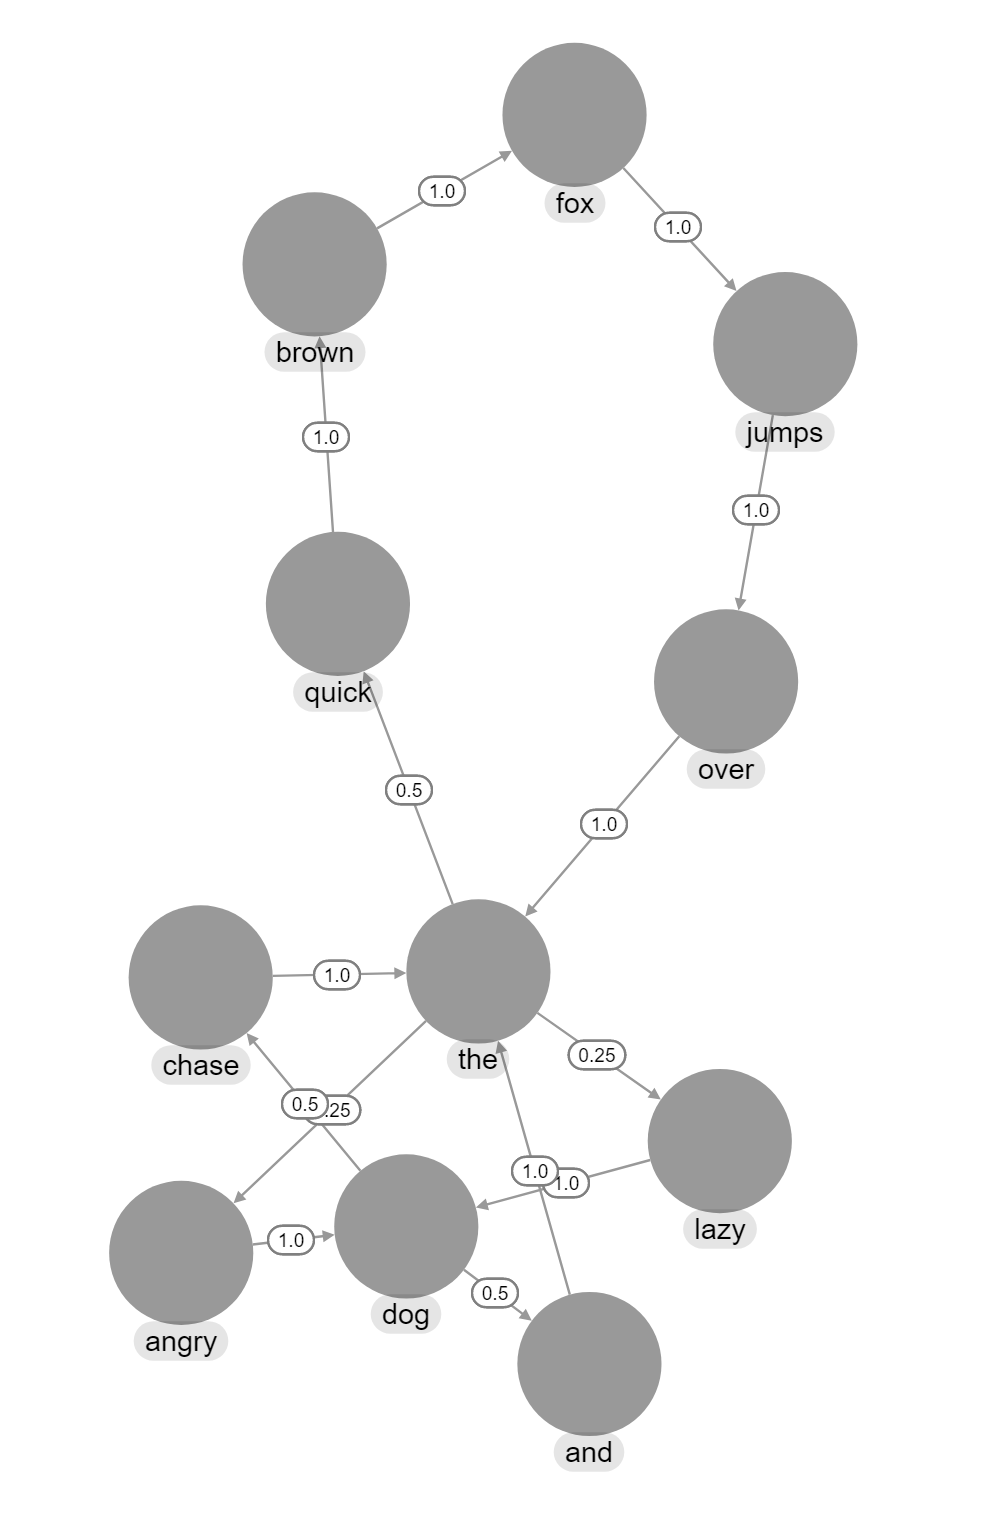
\includegraphics[width=0.75\textwidth]{chain}
    \caption{Przykład łańcucha Markova, dla zdania "The quick brown fox jumps over the lazy dog and the angry dog chase the quick brown fox.", dla wartości $ngram = 1$, oznaczającej stany jako pojedyncze słowama oraz wartoścami prawdopodobieństw przejść pomiędzy stanami obliczonych na podstawie zdania wejściowego.}
    \label{fig:mesh1}
\end{figure}
\FloatBarrier
\subsection{Prawo Zipfa}
Prawo Zipfa to empiryczna obserwacja dotycząca częstotliwości występowania słów w korpusie tekstów. Mówi ono, że jeśli posortujemy słowa występujące w tekście według częstotliwości ich wystąpień i przyporządkujemy każdemu słowu rangę zgodną z jego pozycją w rankingu, to liczba wystąpień słowa o danej randze jest odwrotnie proporcjonalna do wartości tej rangi. W praktyce oznacza to, że najczęściej występujące słowo będzie występować dwa razy częściej niż drugie na liście, trzy razy częściej niż trzecie, i tak dalej. \\
\\
Wykorzystując Prawo Zipfa w generacji tekstów piosenek, można zapewnić, że wygenerowany tekst będzie przypominał rzeczywiste teksty pod względem częstotliwości występowania słów.
\begin{figure}
     \centering
     \begin{subfigure}[b]{0.75\textwidth}
         \centering
         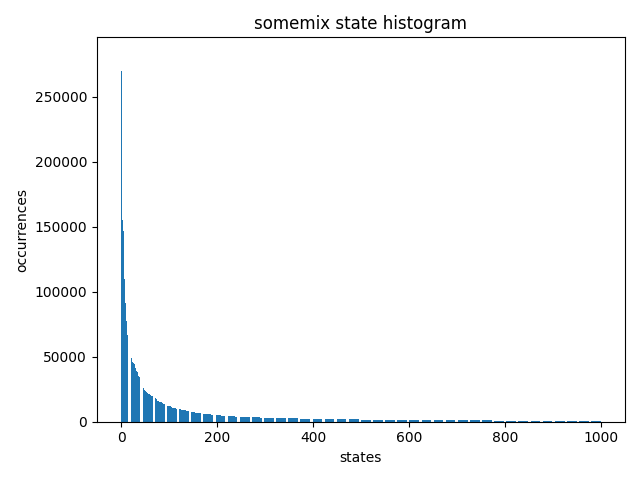
\includegraphics[width=\textwidth]{somemix_zipf1}
         \caption{Wykres 1000 najczęściej pojawiających się słów dla zbioru danych $somemix.csv$.}
         \label{fig:mesh1}
     \end{subfigure}
     \hfill
     \begin{subfigure}[b]{0.75\textwidth}
         \centering
         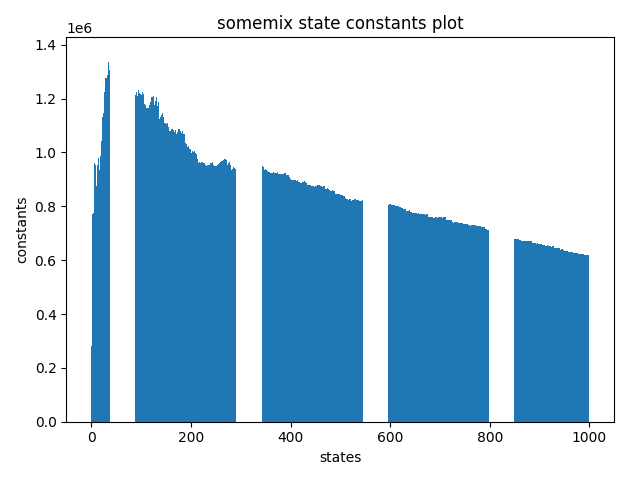
\includegraphics[width=\textwidth]{somemix_zipf2}
         \caption{Wykres stałej $constant = ranga * wystapienia$ dla zbioru danych $somemix.csv$}
         \label{fig:mesh1}
     \end{subfigure}
\end{figure}
\FloatBarrier
\begin{figure}
     \centering
     \begin{subfigure}[b]{0.75\textwidth}
         \centering
         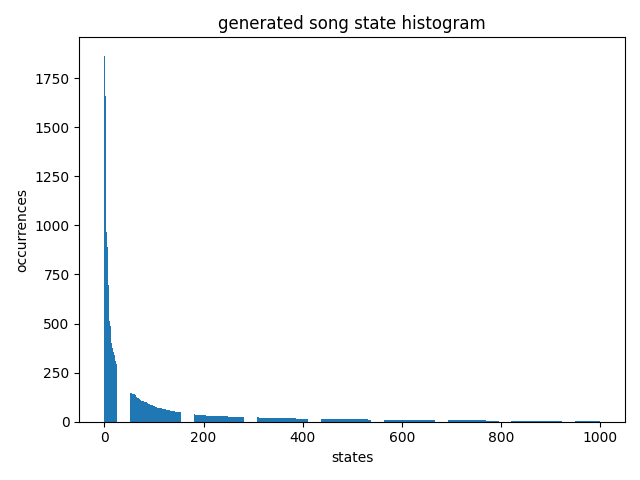
\includegraphics[width=\textwidth]{generated_zipf1}
         \caption{Wykres 1000 najczęściej pojawiających się słów dla piosenki wygenerowanej na podstawie $somemix.csv$ o 100 wersach po 500 słów.}
         \label{fig:mesh1}
     \end{subfigure}
     \hfill
     \begin{subfigure}[b]{0.75\textwidth}
         \centering
         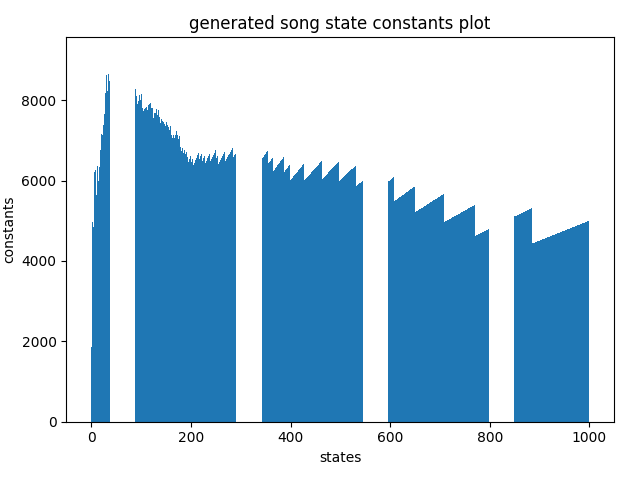
\includegraphics[width=\textwidth]{generated_zipf2}
         \caption{Wykres stałej $constant = ranga * wystapienia$  dla piosenki wygenerowanej na podstawie $somemix.csv$ o 100 wersach po 500 słów}
         \label{fig:mesh1}
     \end{subfigure}
\end{figure}
\FloatBarrier
Podobieństwo wykresów wskazuje na to, że tekst wyjściowy modelu będzie tej samej jakości, przypominając tekst dany na wejściu.
\subsection{Prawo Heapsa}
Prawo Heapsa opisuje zależność pomiędzy wielkością dokumentu w jednostce liter, słów, stanów złożonych ze słów w kontekście liczby unikalnych liter, słów, stanów złożonych ze słów pojawiających się w tekście. Na podstawie prawa, stwierdzamy, że liczba unikalnych stanów rośnie wolniej wraz ze zwiększającą się ilością stanów tekstu, co pozwala nam przewidzieć ilość unikalnych w zasobie danych, co pozwala na lepszą ocenę modelu Markova.
\begin{figure}
     \centering
     \begin{subfigure}[b]{0.49\textwidth}
         \centering
         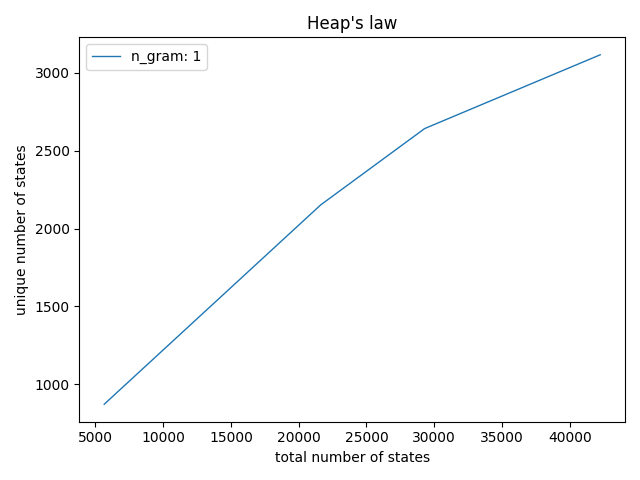
\includegraphics[width=\textwidth]{heaps1}
         \label{fig:mesh1}
     \end{subfigure}
     \hfill
     \begin{subfigure}[b]{0.49\textwidth}
         \centering
         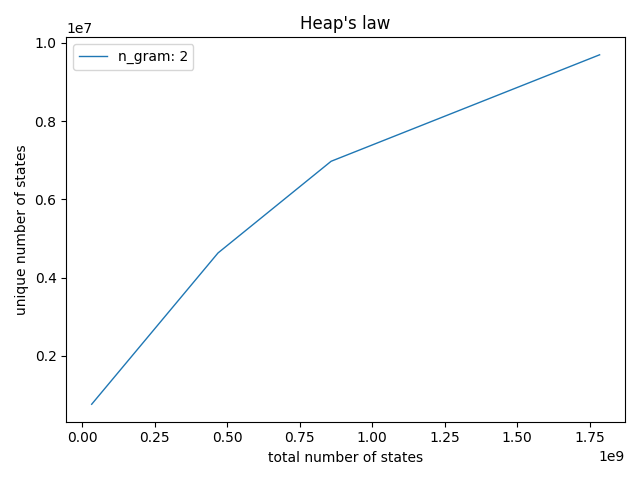
\includegraphics[width=\textwidth]{heaps2}
         \label{fig:mesh1}
     \end{subfigure}
     \hfill
     \begin{subfigure}[b]{0.49\textwidth}
         \centering
         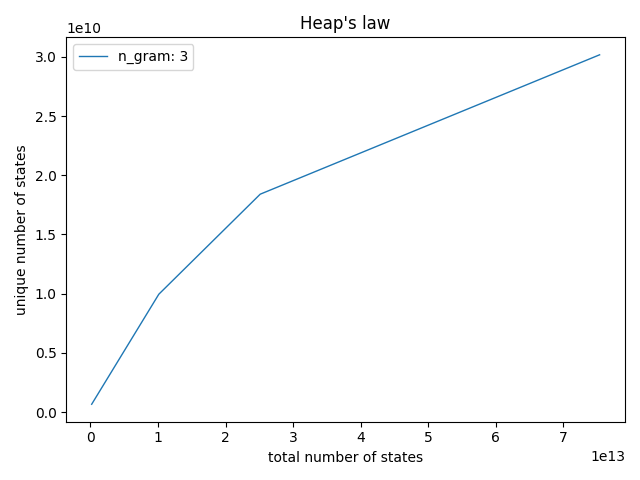
\includegraphics[width=\textwidth]{heaps3}
         \label{fig:mesh1}
     \end{subfigure}
     \hfill
     \begin{subfigure}[b]{0.49\textwidth}
         \centering
         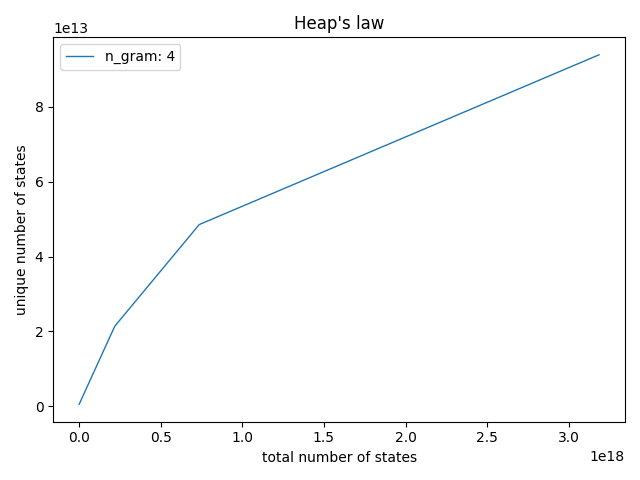
\includegraphics[width=\textwidth]{heaps4}
         \label{fig:mesh1}
     \end{subfigure}
     \hfill
     \begin{subfigure}[b]{0.49\textwidth}
         \centering
         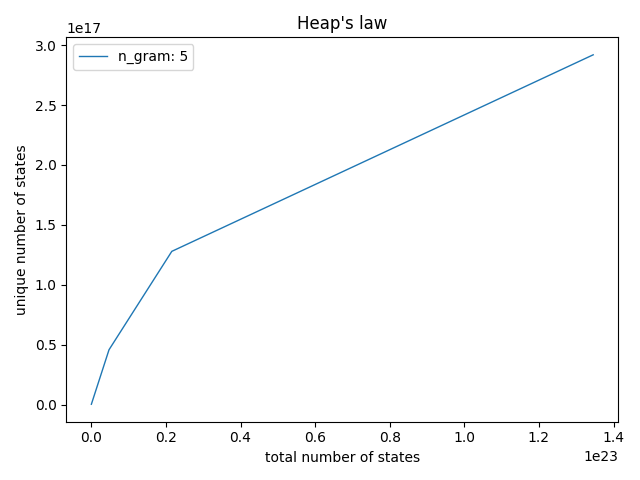
\includegraphics[width=\textwidth]{heaps5}
         \label{fig:mesh1}
     \end{subfigure}
     \hfill
        \caption{Wykres zależności liczby stanów unikalnych od rozmiaru tekstu oraz wartości $ngram$ dla zbiorów danych: $kyuss.csv, led\_zeppelin.csv, Black Sabbath.csv, ac\_dc.csv$.}
        \label{fig:mesh1}
\end{figure}
\FloatBarrier
Prawo Heapsa sprawdza się dla danych. Dodatkowo widzimy, że zmiana jest zależna od $ngramu$. Rośnie ona zwykle wolniej dla większych $ngramow$ co może oznaczać częste pojawianie się w tekstach określonych złożeń słów.
\subsection{Entropia Krzyżowa}
Entropia Krzyżowa to miara zgodności między dwoma rozkładami prawdopodobieństwa. Pozwala określić jak dobrze model generujący tekst przewiduje następny stan na podstawie poprzednich. W przypadku generowania tekstu, entropia krzyżowa może być wykorzystana do oceny jakości generacji. Im mniejsza wartość entropii krzyżowej, tym większa zgodność między rozkładem prawdopodobieństwa generowanego tekstu a rozkładem prawdopodobieństwa prawdziwych tekstów. Pozwala to ocenić czy model tworzy teksty podobne do tych ze zbioru danych, czy też tworzy nowe i oryginalne sentencje.
\\\\
Obliczanie Entropii krzyżowej:
\begin{itemize}
    \item Tworzymy rozkład prawdopodobieństwa wygenerowanego tekstu, zależnie od używanych n-gramów.
    \item Iterując po każdym n-gramie tekstu wygenerowanego obliczamy sumę iloczynów logarytmu prawdopodobieństwa wystąpienia następnego słowa w modelu oraz prawdopodobieństwa wystąpienia następnego słowa w rozkładzie wygenerowanego tekstu. \\\\ $-\sum log(P(M)) * P(L)$ \\ , gdzie $P(M)$ oznacza prawdopodobieństwa wystąpienia następnego słowa w modelu, a $P(L)$ prawdopodobieństwa wystąpienia następnego słowa w rozkładzie wygenerowanego tekstu.
\end{itemize}
\begin{figure}[h]
    \centering
    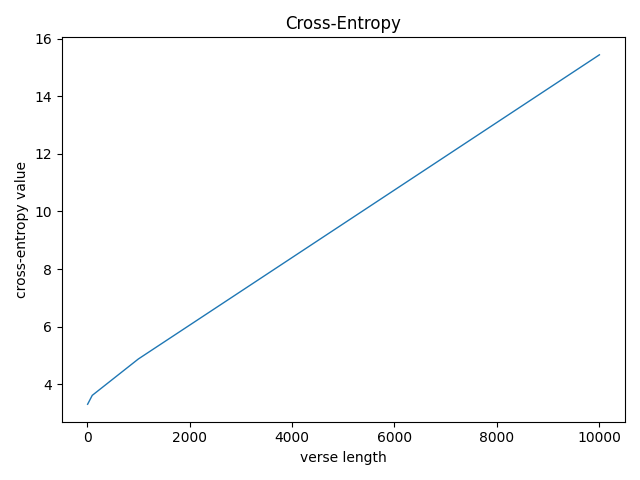
\includegraphics[width=0.75\textwidth]{cross-entropy}
    \caption{Wykres wartości entropii krzyżowej dla tekstu generowanego na podstawie zbioru danych $somemix.csv$, zależnie od rozmiaru wygenerowanego tekstu.}
    \label{fig:mesh1}
\end{figure}
\FloatBarrier
Jak widać, entropia krzyżowa rośnie niemal liniowo względem długości wygenerowanego tekstu. Oznacza to, że model coraz to bardziej generuje tekst niepodobny do oryginalnego zależnie od długości wygenerowanego tekstu.
\subsection{Perpleksja}
Perpleksja to stopień trudności zrozumienia tekstu, miara nieprzewidywalności modelu. Im niższa tym tekst bardziej przypomina oryginalny i jest bardziej kreatywny. Aby policzyć wartość perpleksji tekstu korzystamy ze wzoru: $Perplexity(M) = 2^{H(L,M)}$ gdzie $M$ oznacza model, $L$ oznacza wygenerowany tekst, a $H(L, M)$ wartość entropii krzyżowej.
\begin{figure}[h]
    \centering
    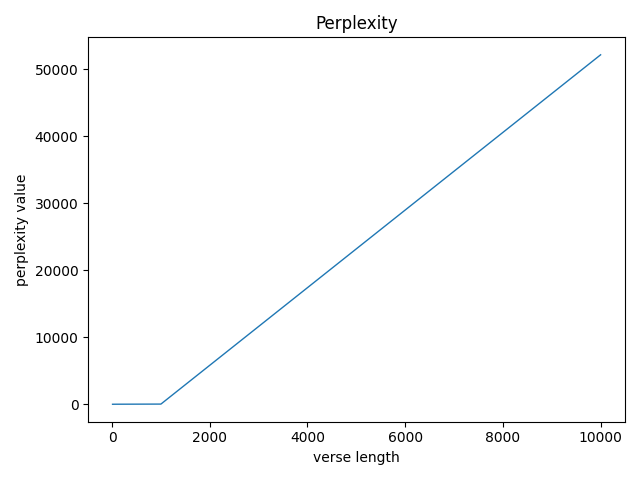
\includegraphics[width=0.75\textwidth]{perplexity}
    \caption{Wykres wartości perpleksji dla tekstu generowanego na podstawie zbioru danych $somemix.csv$, zależnie od rozmiaru wygenerowanego tekstu.}
    \label{fig:mesh1}
\end{figure}
\FloatBarrier
Jak widać, wykresy eksperymentu dla entropii krzyżowej i perpleksji się nie różnią, ponieważ w gruncie rzeczy znaczą tą samą miarę.
\subsection{Self-BLEU}
Self-BLEU określa różnorodność generowanego tekstu. Wykorzystuje wskaźnik \href{https://pl.wikipedia.org/wiki/BLEU}{BLEU} (ang. BiLingual Evaluation Understudy), licząc jego wartość dla kombinacji par wszystkich unikalnych sentencji wygenerowanego tekstu, w tym przypadku wersów piosenki, otrzymując końcowo ich średnią. Im mniejsza wartość wskaźnika tym większa różnorodność w tekście. Metryka pozwala uniknąć monotonności tekstu. \\\\
Sam wskaźnik BLEU mierzy podobieństwo między tłumaczeniem maszynowym a jednym lub wieloma tłumaczeniami referencyjnymi poprzez porównanie stopnia pokrycia n-gramów (ciągów po n kolejnych słów) między nimi. Im wyższy wynik, tym większe podobieństwo między tłumaczeniem a referencją. Wartości wskaźnika BLEU mieszczą się w przedziale od 0 do 1, gdzie 1 oznacza idealne dopasowanie tłumaczenia maszynowego do referencji. W praktyce, oczekuje się wyników BLEU powyżej 0,4-0,5, aby uznać tłumaczenie maszynowe za akceptowalne.\\
\begin{figure}[h]
    \centering
    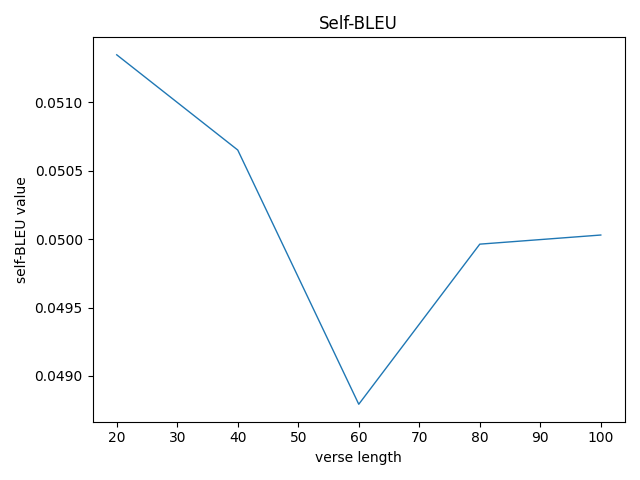
\includegraphics[width=0.75\textwidth]{self-bleu}
    \caption{Wykres wartości Self-BLEU dla tekstu generowanego na podstawie zbioru danych $somemix.csv$, zależnie od rozmiaru wygenerowanego tekstu.}
    \label{fig:mesh1}
\end{figure}
\FloatBarrier
Jak widać, tekst zachowuje wysoką różnorodność, poprzez losowy wybór początku wersu rozkładem równomiernym, a z coraz to większym rozmiarem tekstu napotykamy na nowe frazy, co zwiększa jego różnorodność, jednak wciąż wynik jest zależny od wygenerowanych tekstów.
\FloatBarrier
\subsection{Przykładowe wyniki}
\newpage
\begin{center}
    Przykładowe wyniki generacji 10 wersów po 10 słów dla zbioru danych $english\_mixtape.csv$: \\
    \leavevmode\\
    \textsl{Shy yeah repeat everything i want you hard dont get \\
            Slow with plenty of desperation in the night end of \\
            Until that day lost my way you bat your eyes \\
            Back baby cause your man is back wonder where you \\
            Under water forever was their faith i will let you \\
            Windows feel like giving up cause you know theres only \\
            Lets shout lets make it baby now worry like lying \\
            Some room for you and me can you heal what \\
            Shot cmon terminator uzi makers regulators gon na blow my \\
            A poto over the road youre on your move what} \\
    \leavevmode\\\leavevmode\\
    Przykładowe wyniki generacji 10 wersów po 10 słów dla zbioru danych $somemix.csv$: \\
    \leavevmode\\
    \textsl{Hell forget about me making a movie turn on a \\
            Bas en haut jaimais manger sa peau je sais que \\
            Main banu tera ehsaas main yaar banavanga akhiyaan milavanga akhiyaan \\
            So stroke me and no reason to believe that parted \\
            Now sexy dance sexy dancer hot as hades early eighties \\
            How sophisticated you know what they do they laugh and \\
            Of brotherly love the feel of silk and your talents \\
            Goddamn alotta brilliant bitch have it you be not much \\
            Line trill tell me youre always gon na need your \\
            Crawling on them haters sick itd be worth more dan} \\
    \leavevmode\\\leavevmode\\
\end{center}
\section{Rekurencyjne Sieci Neuronowe}
\end{document}
